\documentclass[onecolumn]{article} %[twocolumn]
\usepackage[utf8]{inputenc}
\usepackage[margin=0.8in]{geometry} %Margins
\usepackage{multicol} %Columns: multiples
\usepackage[hidelinks]{hyperref} %Hyperlinks
\usepackage{authblk} %Authors: affiliation
\renewcommand\Affilfont{\itshape\small} %Authors: affiliation font
\usepackage{tabularx} % Tabular: automatic line-break
\usepackage[justification=raggedright]{caption} %Floats: caption as with tables
\usepackage{ltablex} %Floats: long
\renewcommand{\arraystretch}{1.5} %Tables: more space between rows
\usepackage{graphicx} %Figures: import
\graphicspath{{figures/}} %Figures path
\usepackage{subcaption} %Figures: multiple with one caption
\usepackage{amsmath} %Case definition
\usepackage[toc,page]{appendix} %Appendix
\newenvironment{conditions} %Conditions
{\par\vspace{\abovedisplayskip}\noindent\begin{tabular}{>{$}l<{$} @{${}={}$} l}} %Conditions
{\end{tabular}\par\vspace{\belowdisplayskip}} %Conditions
\usepackage{natbib} %Citations: APA
\usepackage{amsmath} %Use \[ ... \]
\usepackage{xcolor} %colors
\usepackage{import}

\title{Food web aggregation: effects on key positions}
\author[1]{Emanuele Giacomuzzo}
\author[1]{Ferenc Jordàn}
\affil[1]{Stazione Zoologica Anton Dohrn, Napoli, 80122, Italy}
%\affil[2]{Central European University, Budapest, 1051, Hungary}
\date{}
\begin{document}
\maketitle

\subimport{sections/}{introduction.tex}

						\begin{figure}[htbp]%{\textwidth}
							\centering
							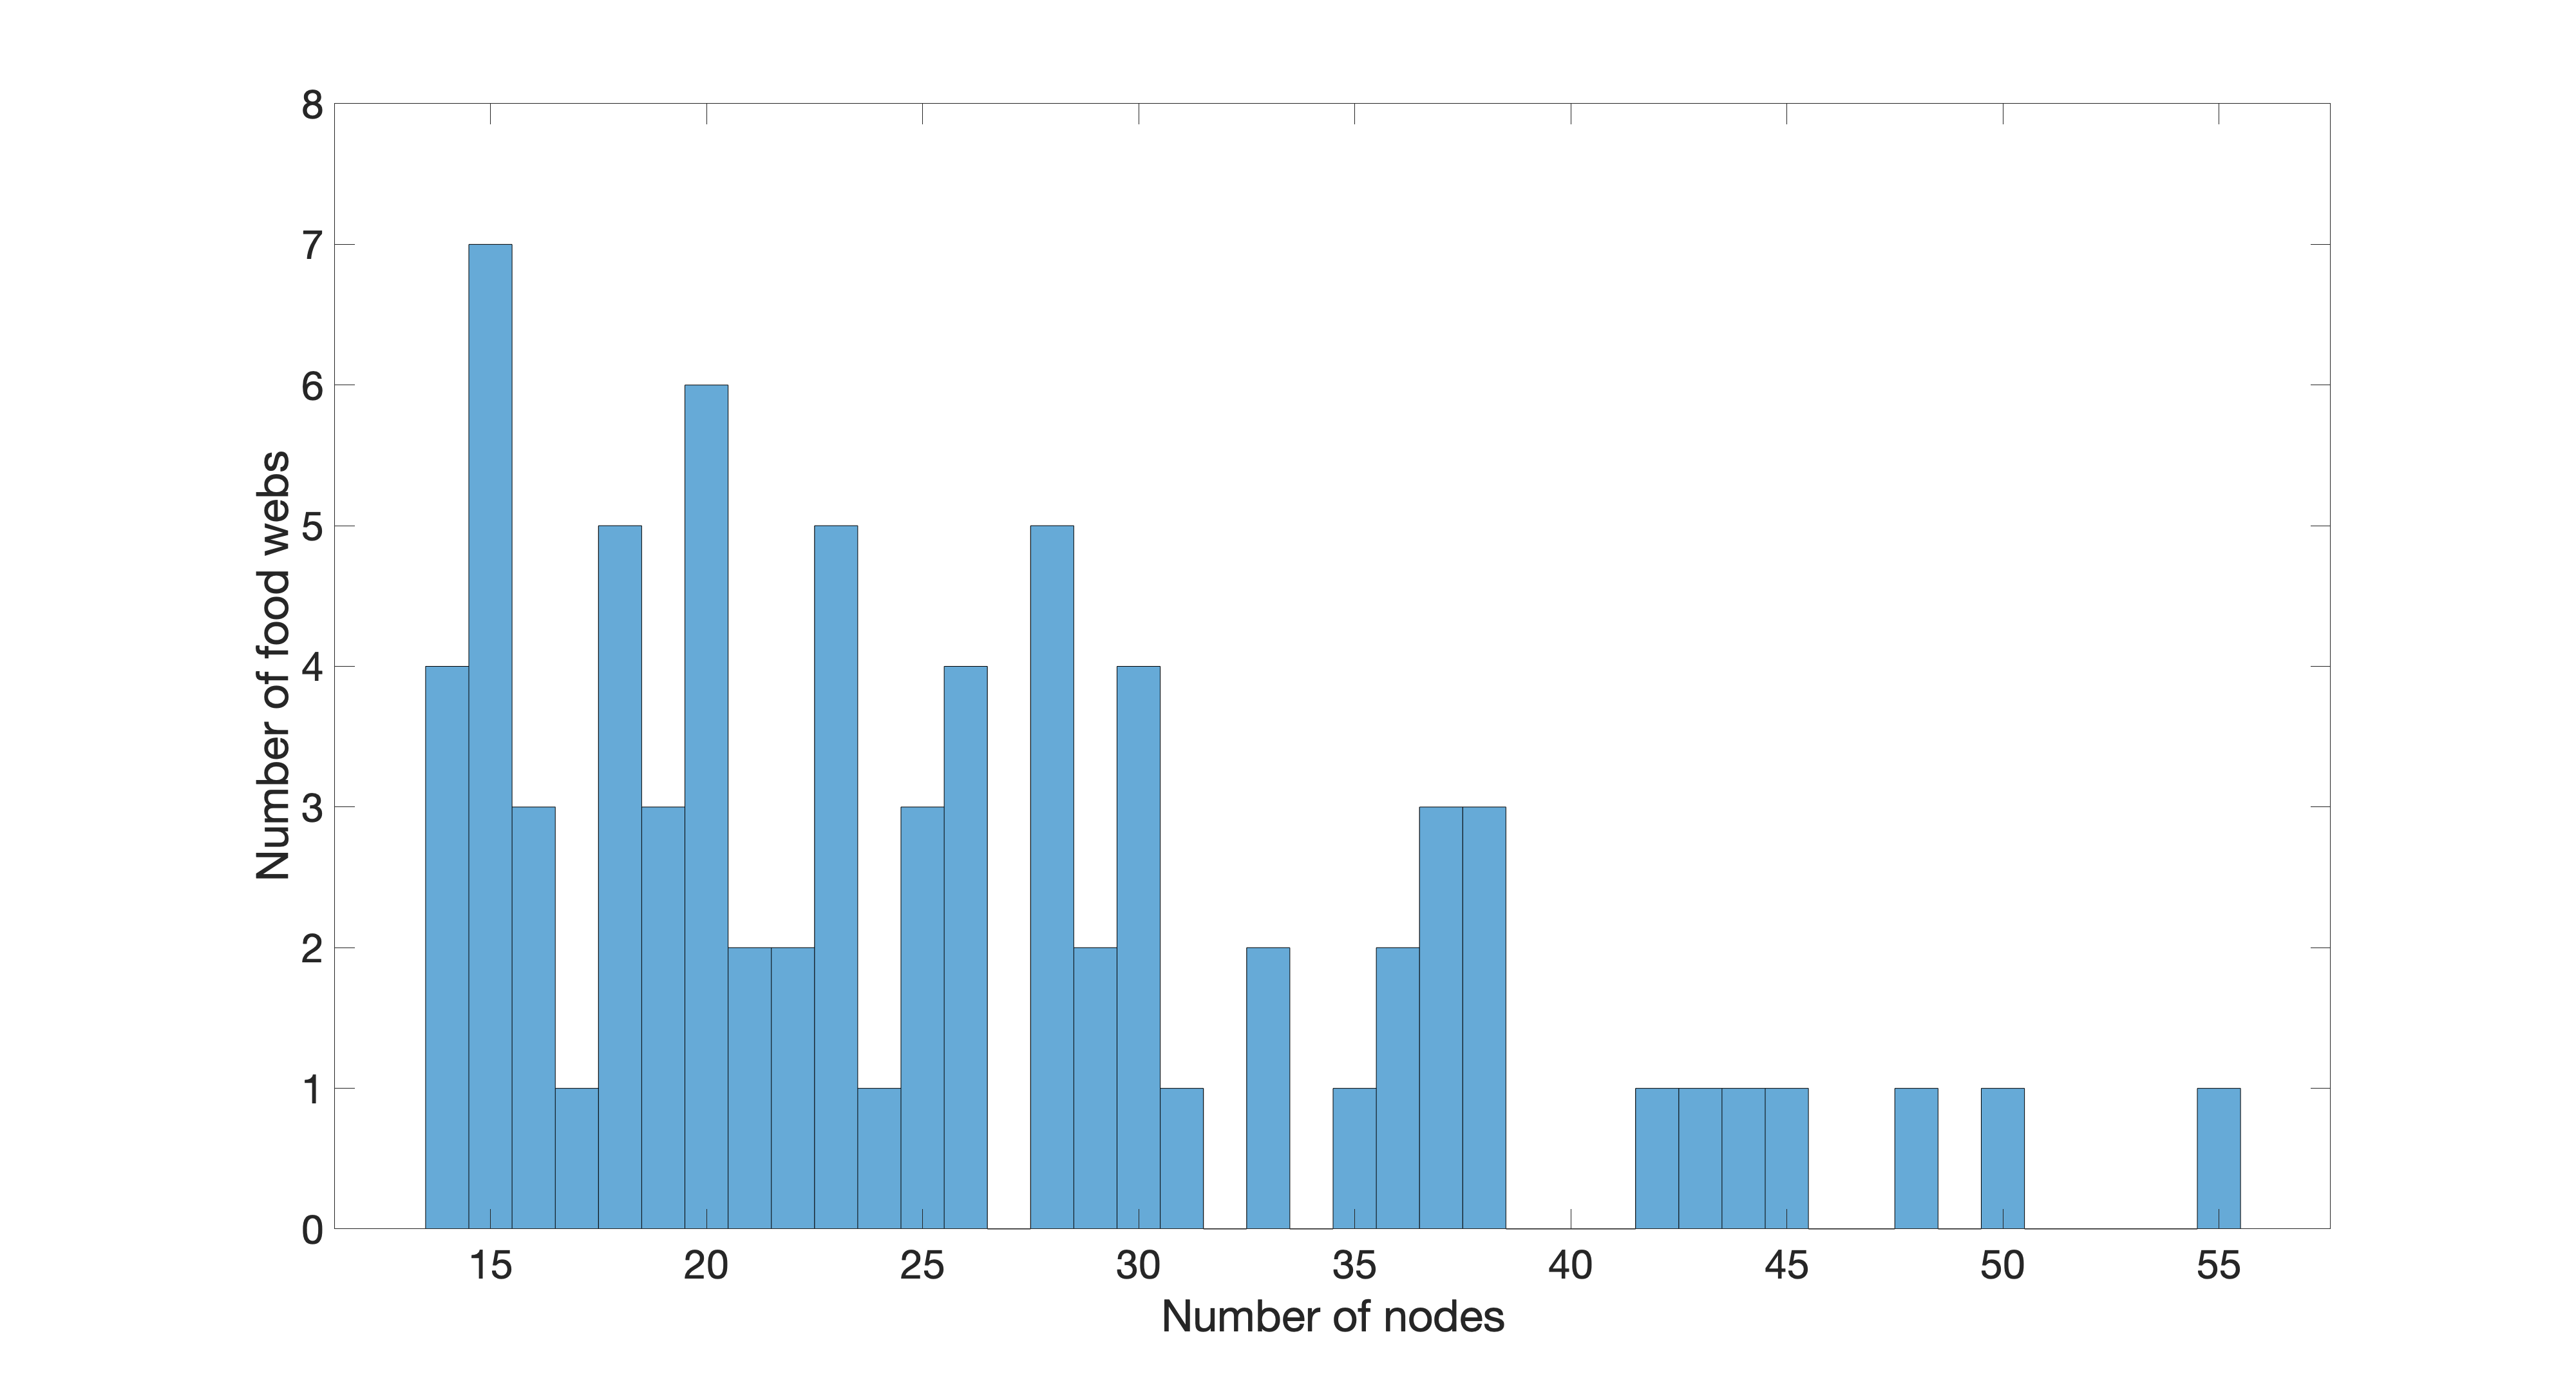
\includegraphics[width=1.0\linewidth]{food_web_sizes.png}
							\caption{ \subimport{captions/}{caption_food_web_sizes.txt} }
							\label{fig:equivalences}
						\end{figure} %CHANGE

\subimport{sections/}{methods.tex}
\subimport{sections/}{results.tex}

						\begin{figure}[htbp]%{\textwidth}
							\centering
							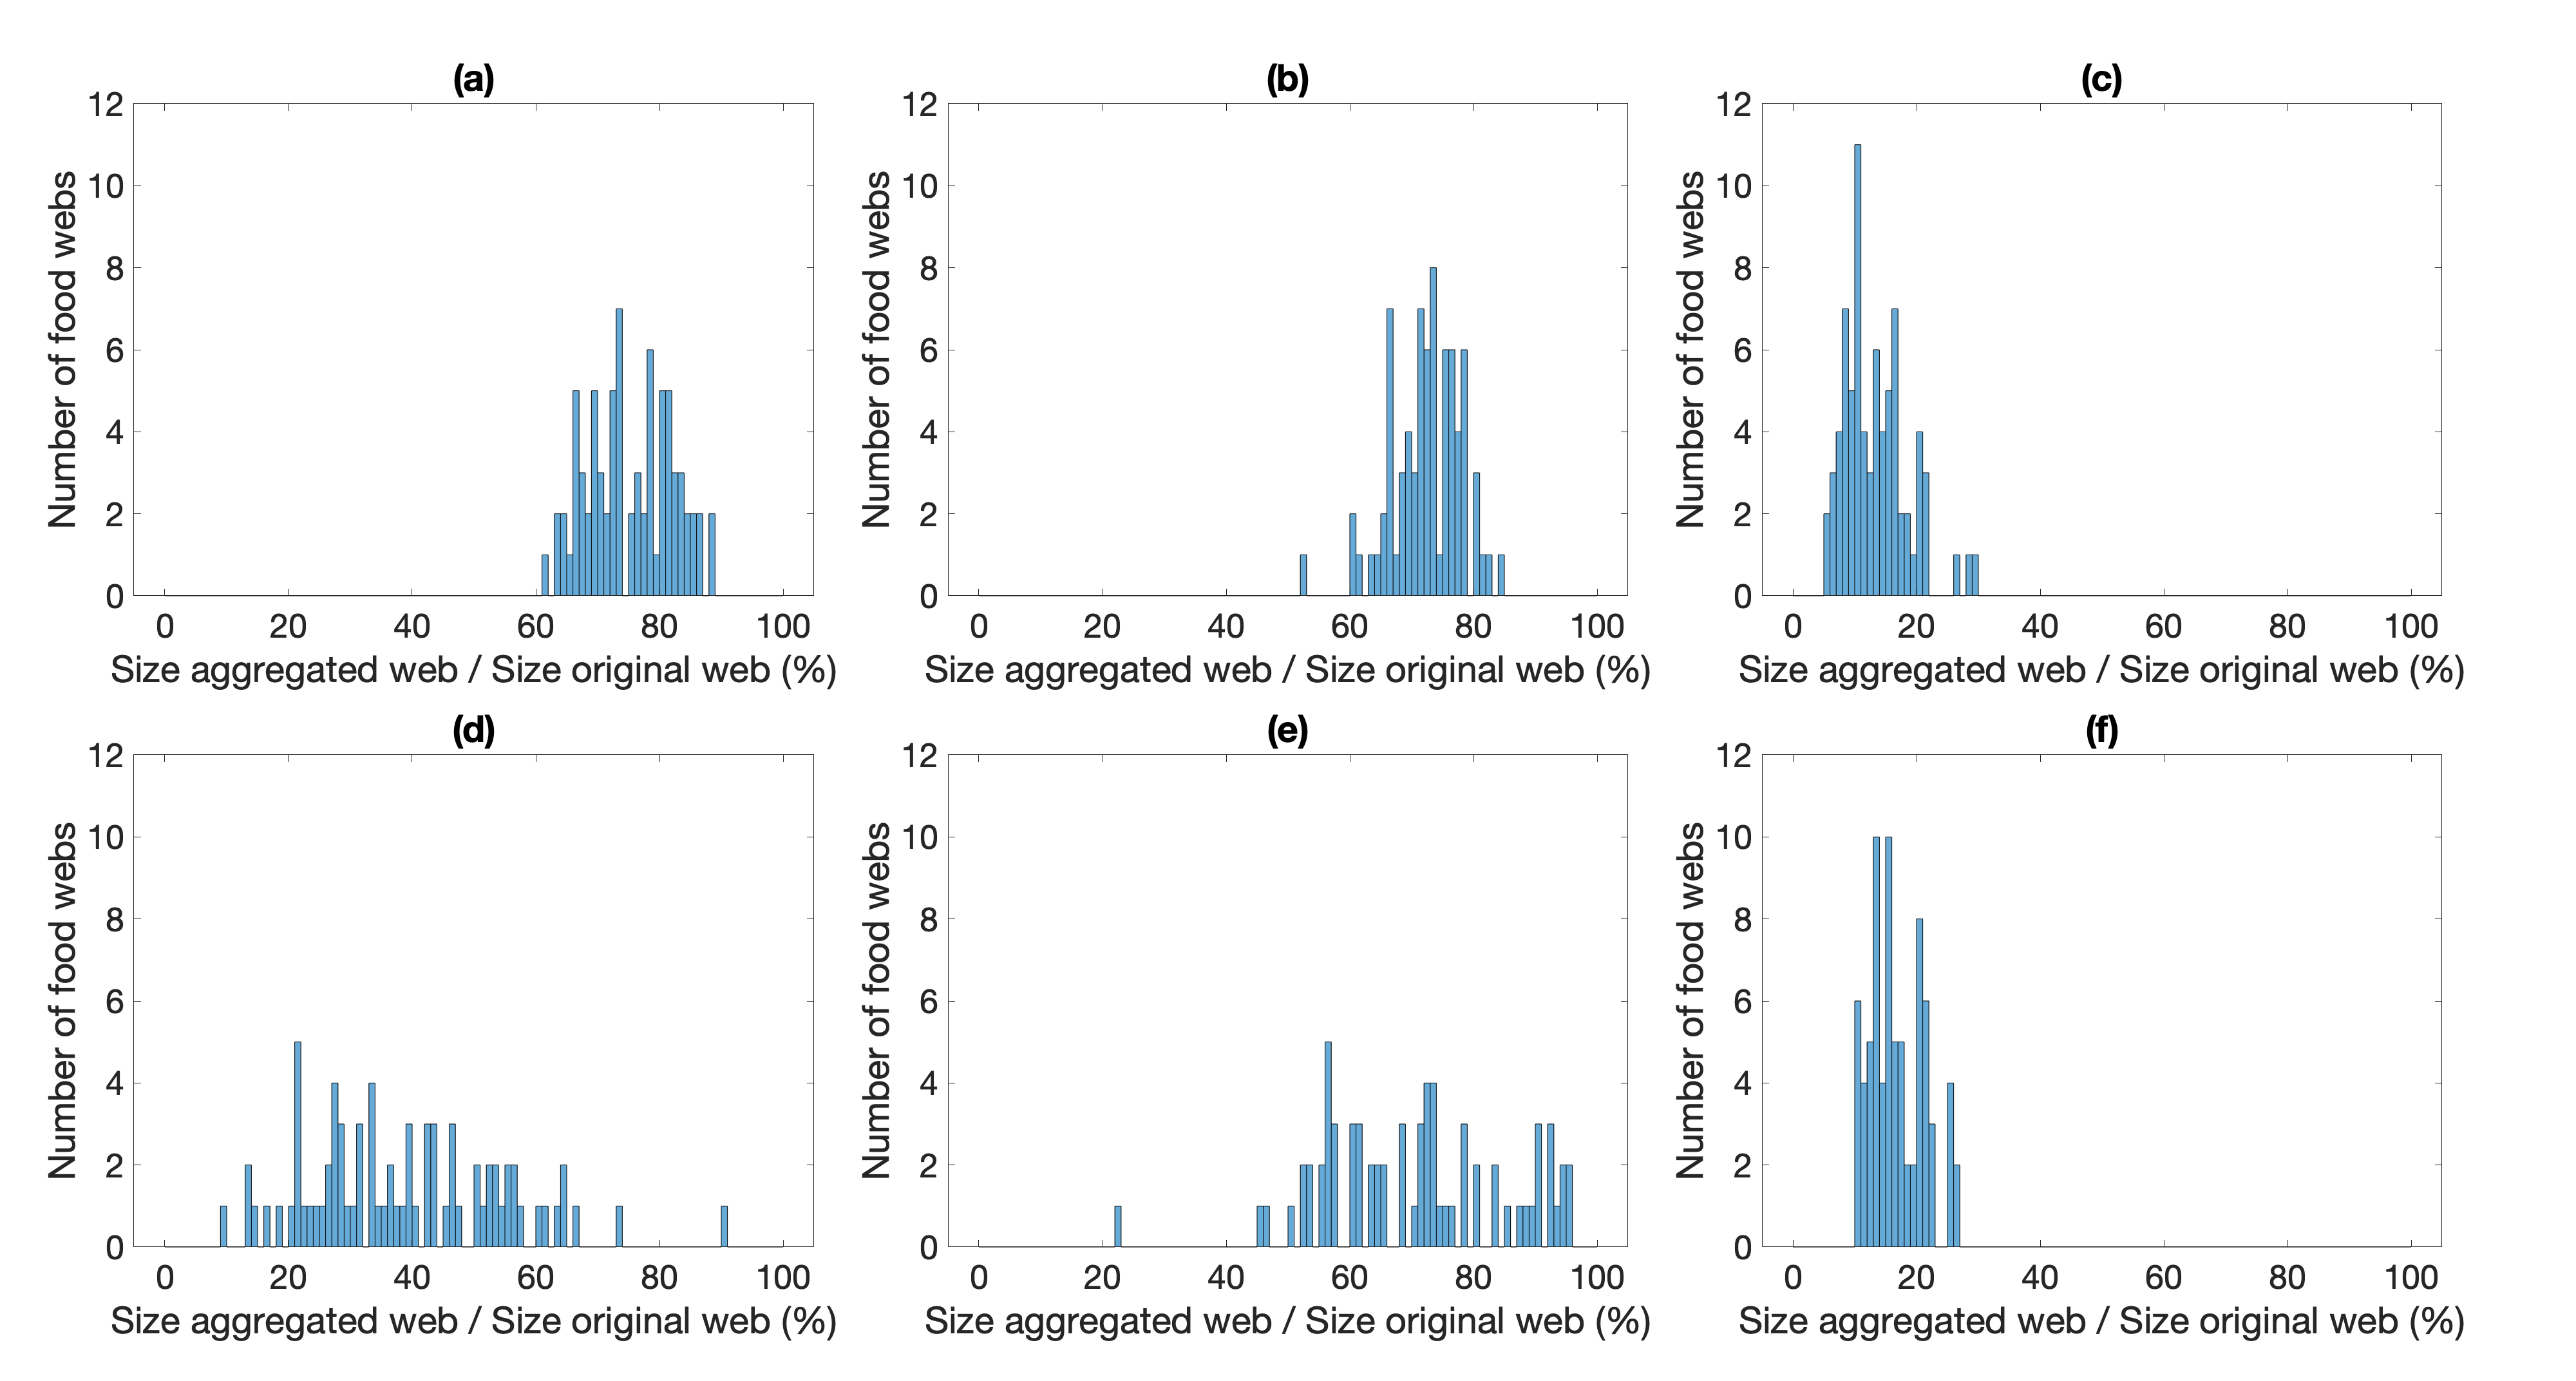
\includegraphics[width=1.0\linewidth]{cluster_sizes.png}
							\caption{ \subimport{captions/}{caption_cluster_sizes.txt} }
							\label{fig:equivalences}
						\end{figure} %CHANGE

						\begin{figure}[htbp]%{\textwidth}
							\centering
							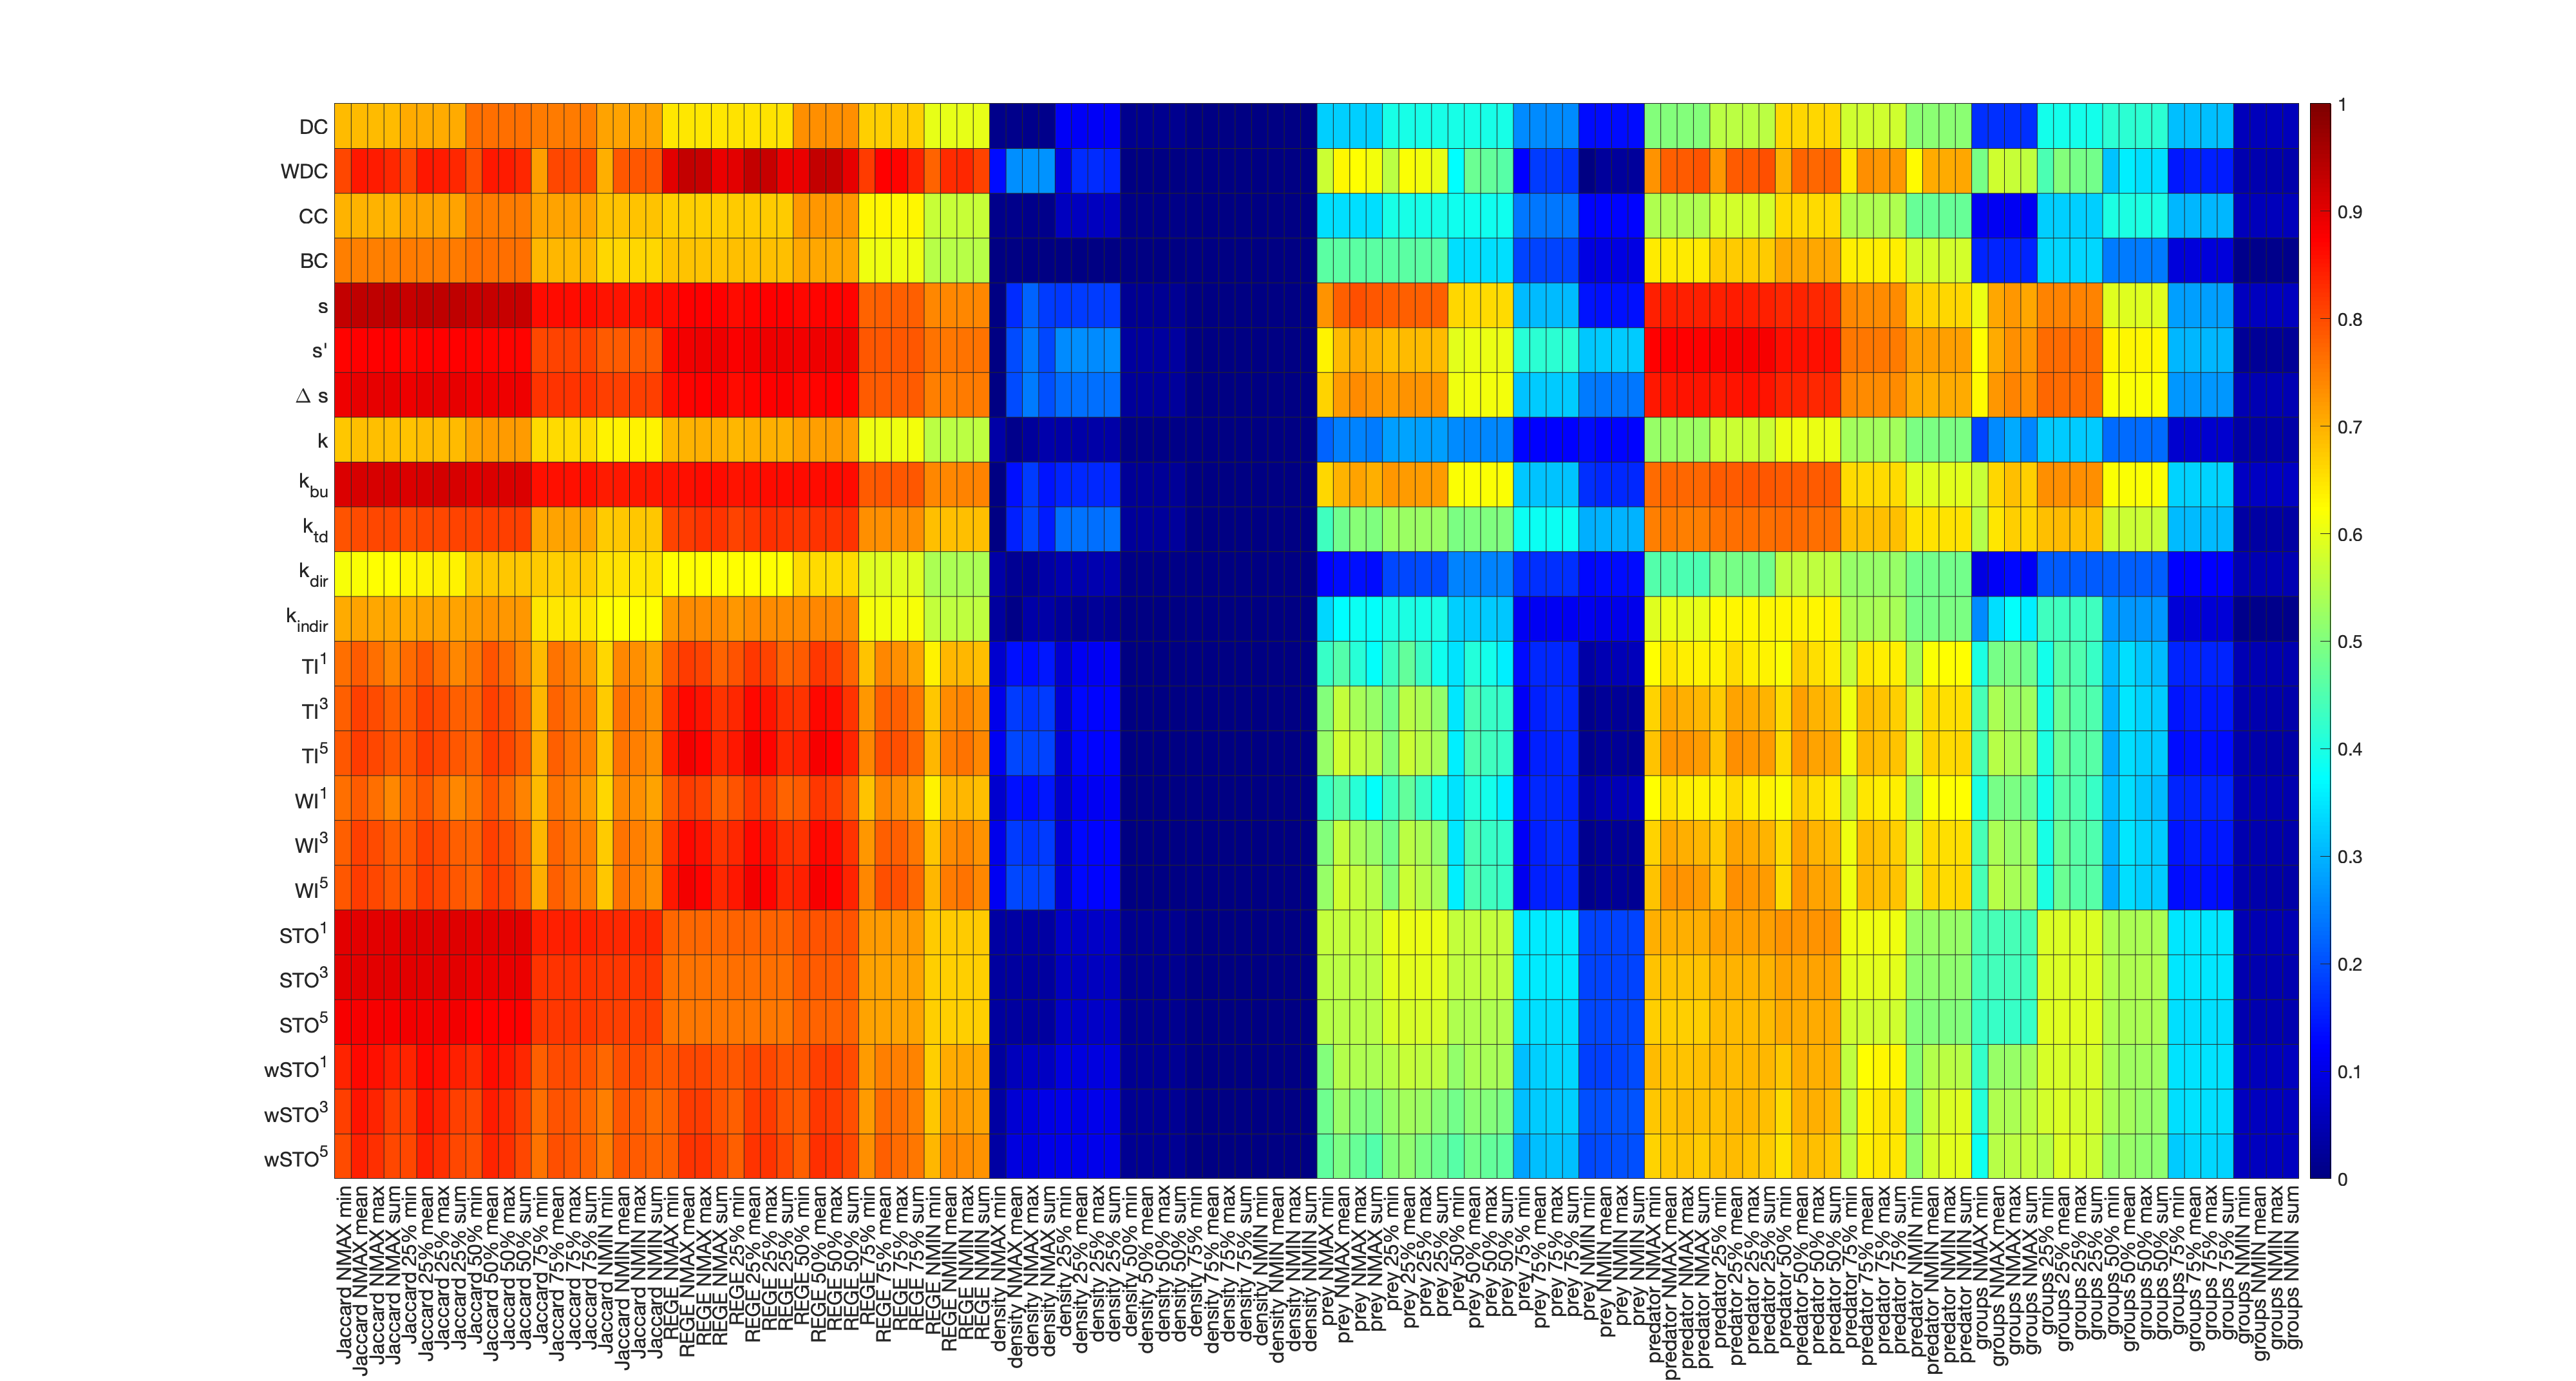
\includegraphics[width=1.0\linewidth]{mean_kendalls_a.png}
							\caption{ \subimport{captions/}{caption_mean_kendalls.txt} }
							\label{fig:equivalences}
						\end{figure} %CHANGE

						\begin{figure}[htbp]%{\textwidth}
							\centering
							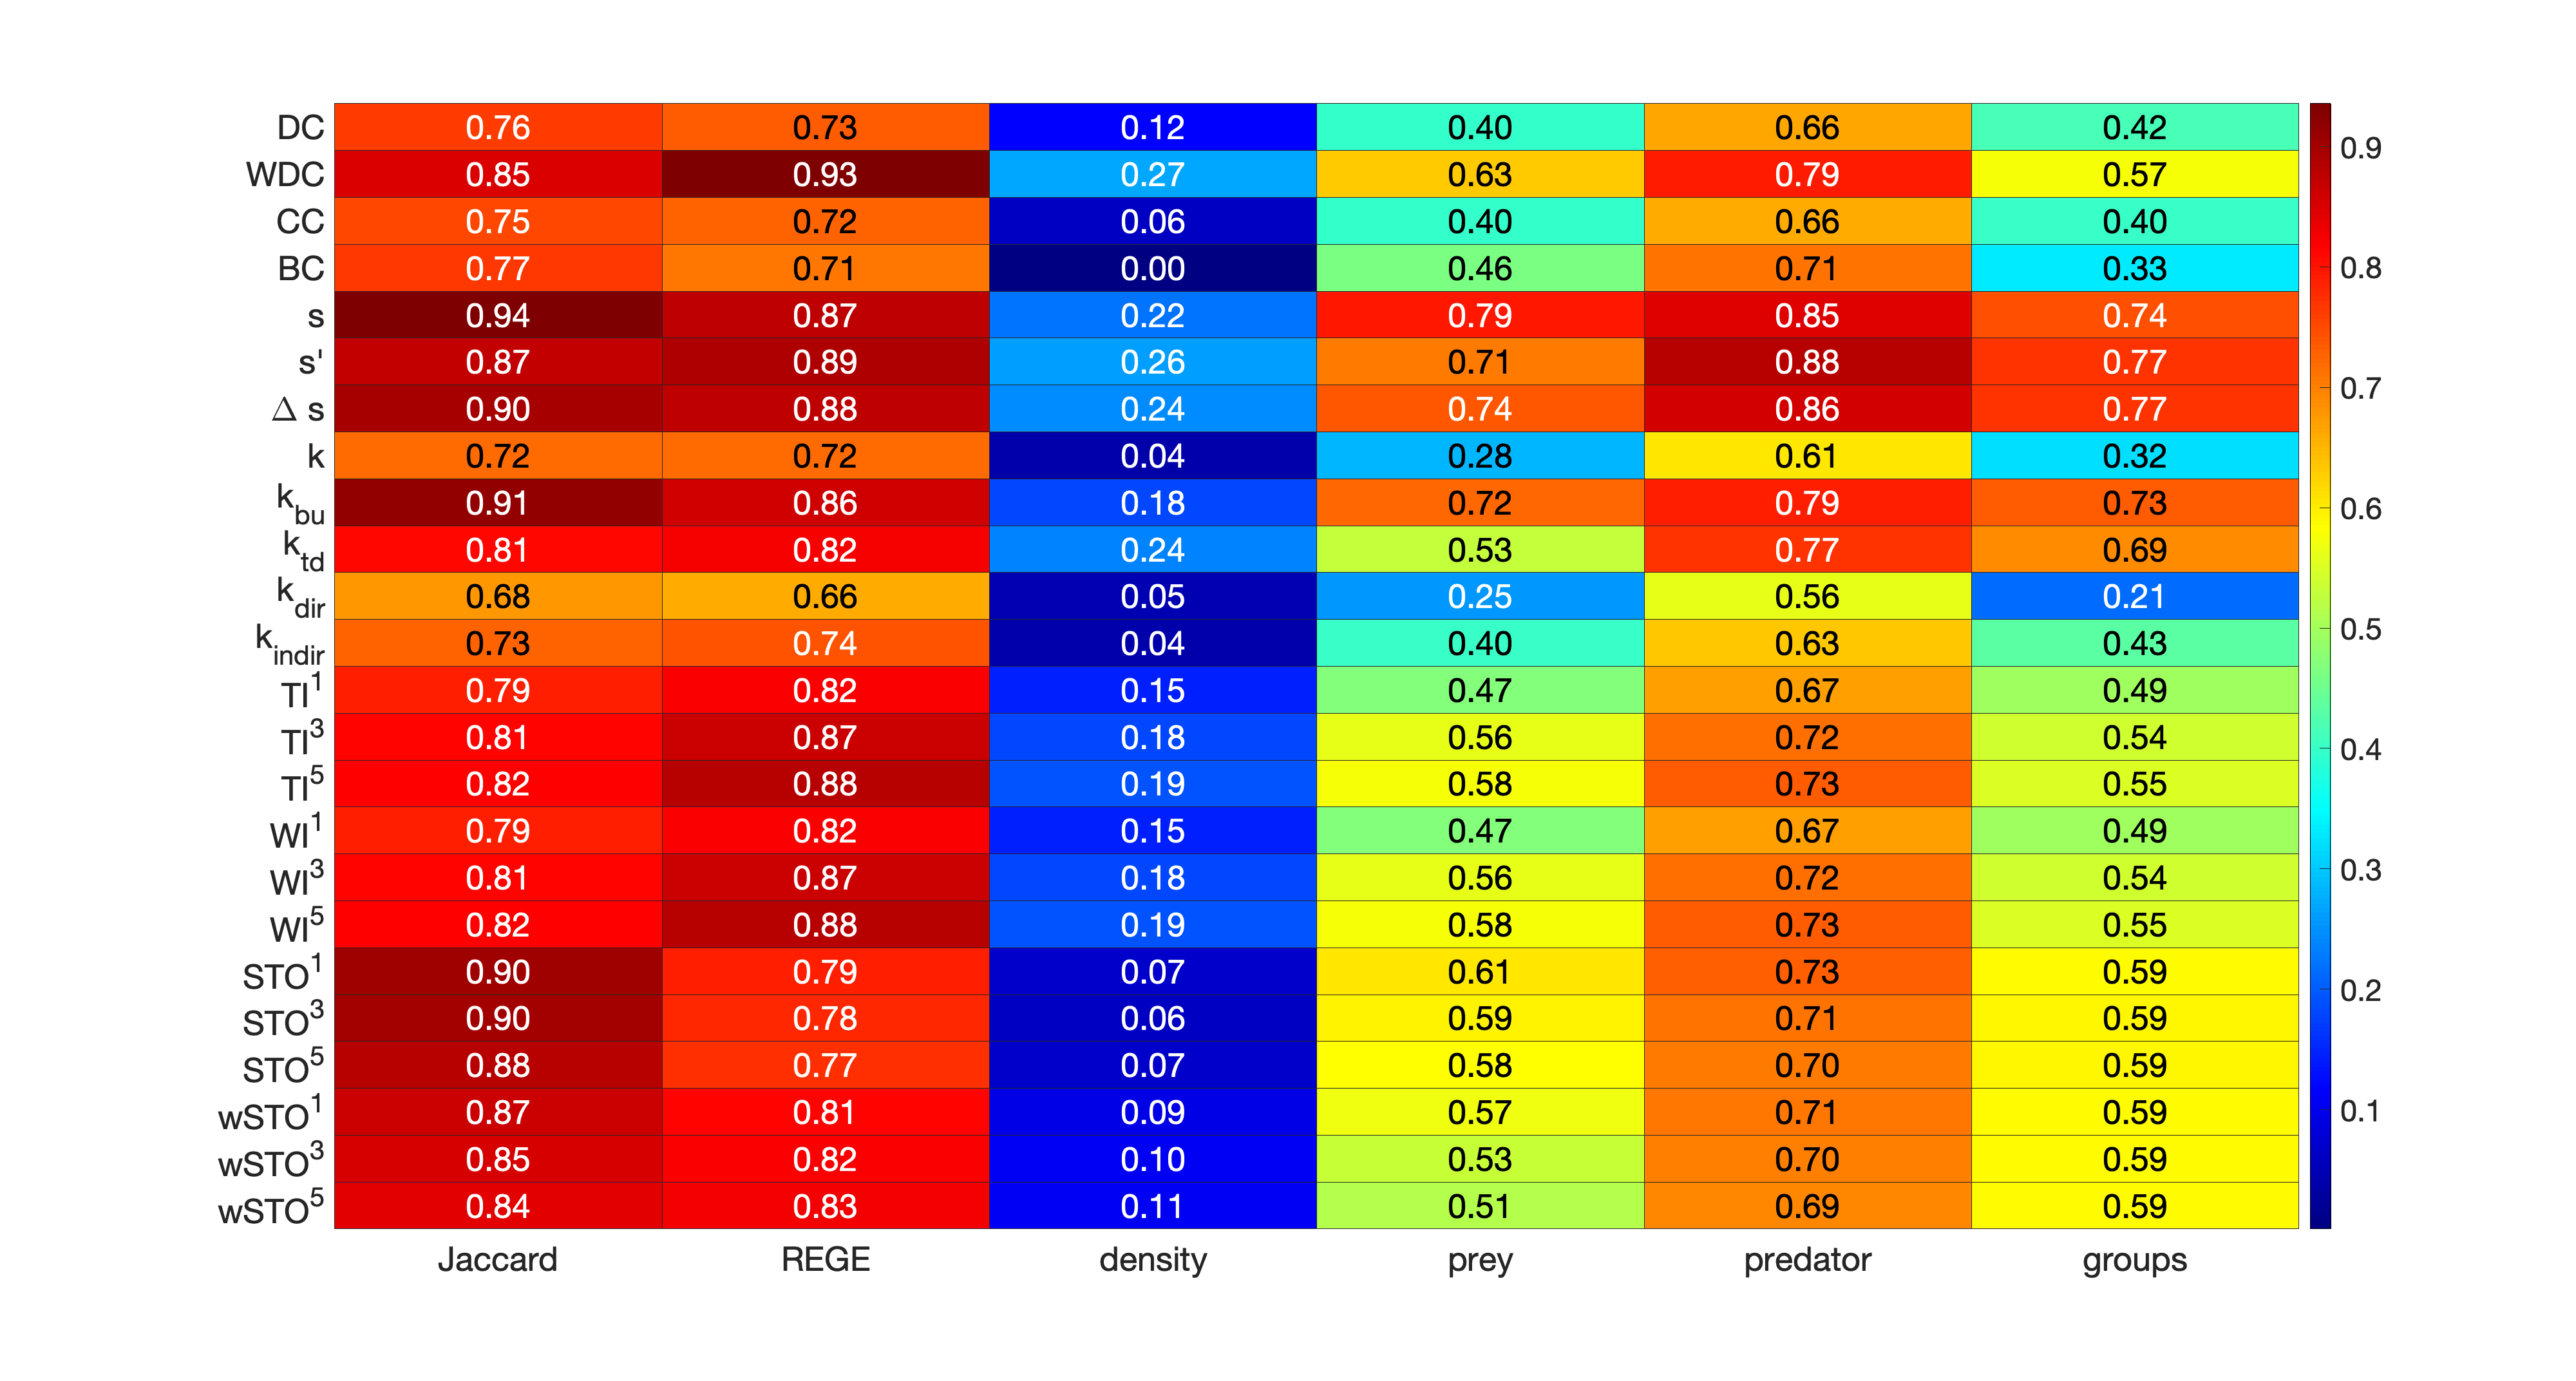
\includegraphics[width=1.0\linewidth]{best_kendalls.png}
							\caption{ \subimport{captions/}{caption_best_kendalls.txt} }
							\label{fig:equivalences}
						\end{figure} %CHANGE

						\subimport{tables/}{rank_table.tex}

\subimport{sections/}{acknowledgments.tex}
\subimport{sections/}{supplementary_material.tex}
\bibliographystyle{apalike}
\bibliography{/Applications/Mendeley/library.bib}
\onecolumn
\begin{appendices}
	\section{Hierarchical clustering with Jaccard index} \label{appendix:jaccard}
	\subimport{sections/}{Jaccard_algorithm.tex}
	\section{Hierarchical clustering with REGE index} \label{appendix:rege}
	\subimport{sections/}{rege_algorithm.tex}
	\section{Topological importance computation} \label{appendix:TI}
	\subimport{sections/}{TI_algorithm.tex}
	\section{Trophic field overlap computation} \label{appendix:TO}
	\subimport{sections/}{TO_algorithm.tex}
\end{appendices}

\end{document}
